\subsection{miniWECC-AGC - WIP} 
Multi area agc using optional VTS in PSTv4.
Two different area configurations: One is the same as used PSLTDSim examples, and one made to mimic EIA regions.
Example allows for comparing VTS to FTS simulation methods.

\noindent Elapsed Time (FTS):	 1027.2399\\
Elapsed Time (VTS):	 189.9163\\
VTS speed up: 5.4089\\

DC lines are modeled as power injection via load settings.
This power import/export is \textbf{not} included in AGC calculations.

\begin{figure}[H]
	\centering
	\footnotesize
	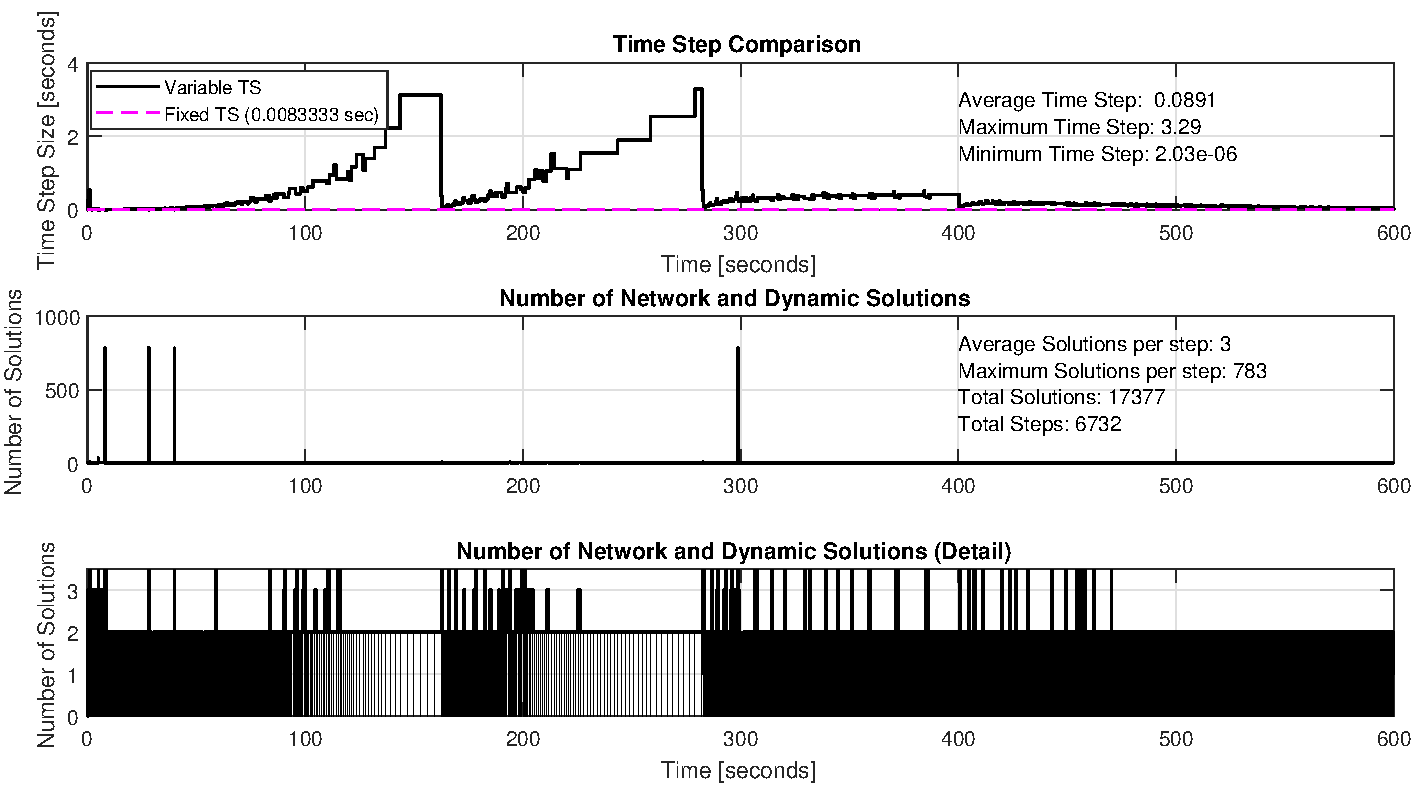
\includegraphics[width=\linewidth]{examples/miniWECC/mwAGC-timestep}
	\caption{MiniWECC AGC recovery FTS vs VTS time step size and solution count.}
	\label{fig: mwAGC steps}
\end{figure}%\vspace{-1 em}


\begin{figure}[H]
	\centering
	\footnotesize
	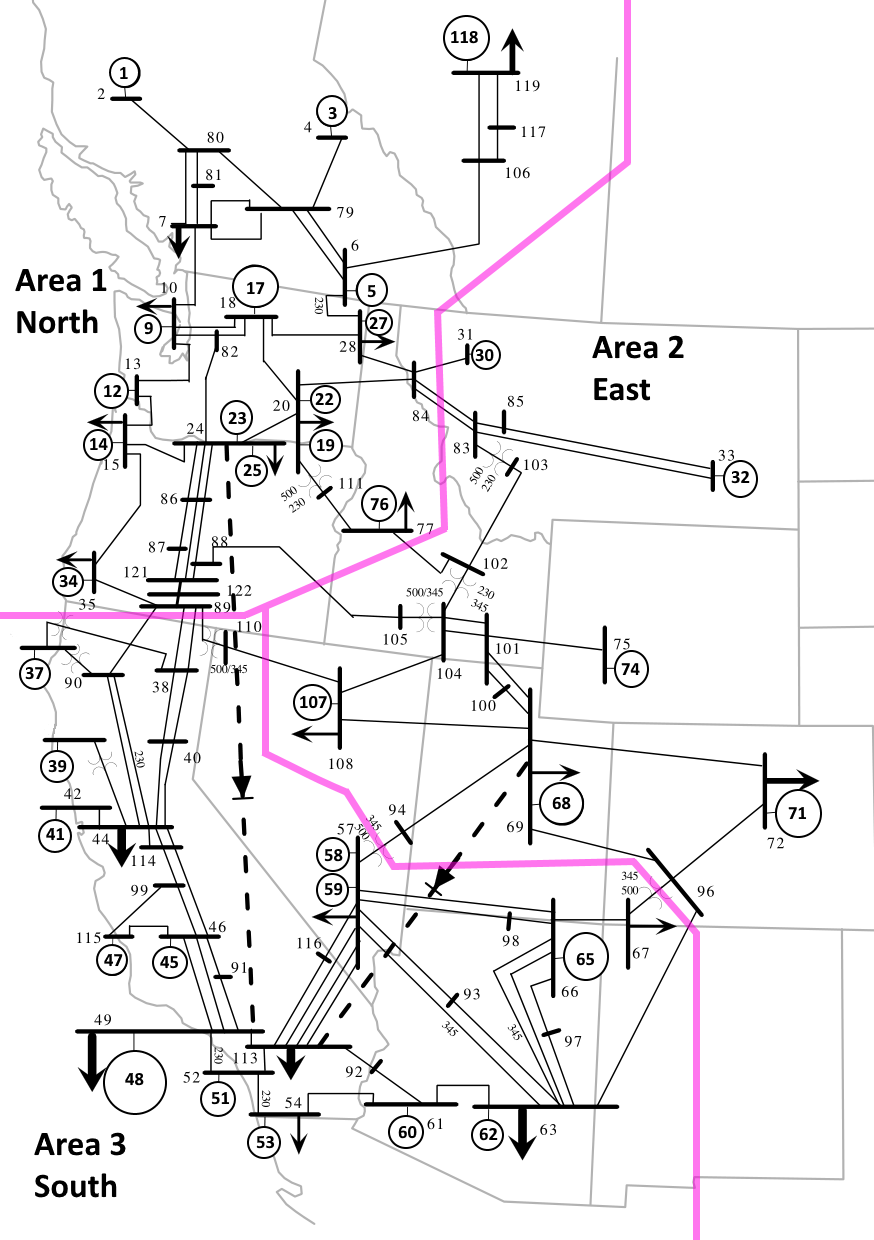
\includegraphics[width=\linewidth]{examples/miniWECC/miniWECC-split03-PSLTDSim}
	\caption{MiniWECC using PSLTDSim Areas.}
	\label{fig: mw area option 1}
\end{figure}%\vspace{-1 em}

\begin{figure}[H]
	\centering
	\footnotesize
	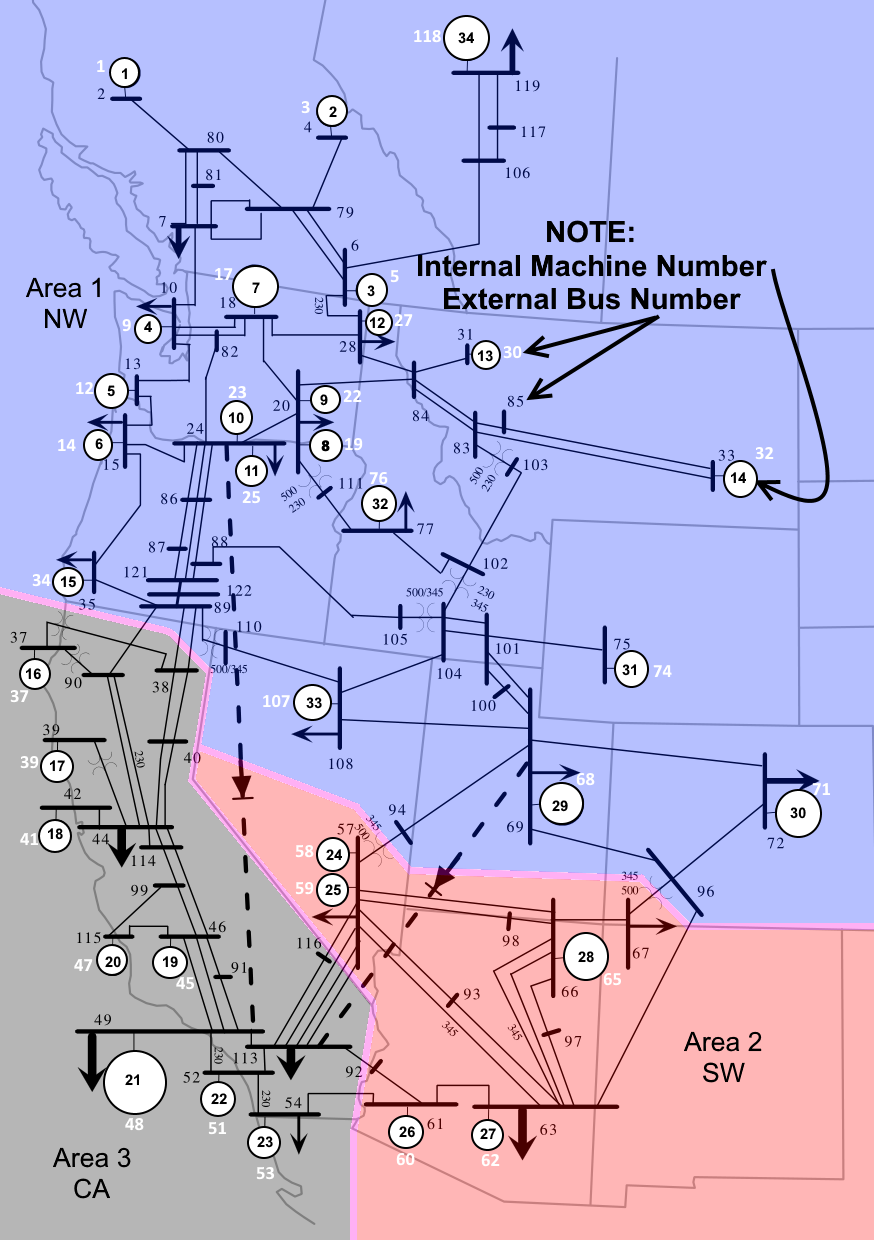
\includegraphics[width=\linewidth]{examples/miniWECC/miniWECC-split03-EIA}
	\caption{MiniWECC using EIA Area Approximation.}
	\label{fig: mw area option 2}
\end{figure}%\vspace{-1 em}


\begin{figure}[H]
	\centering
	\footnotesize
	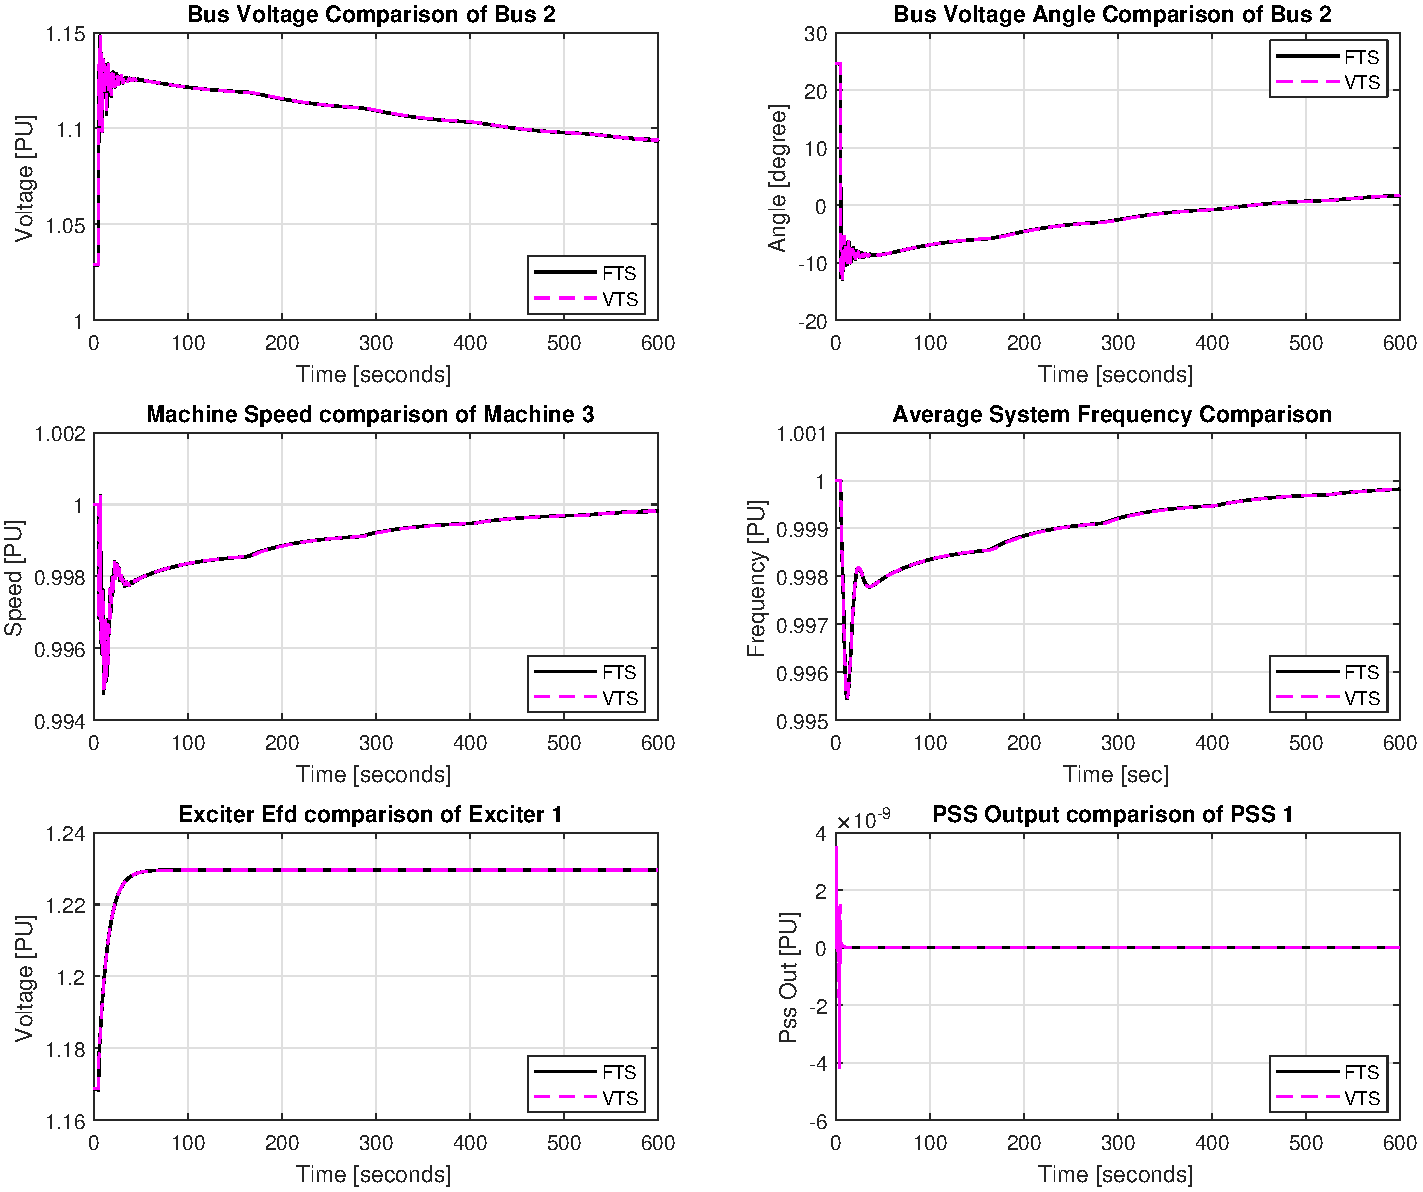
\includegraphics[width=\linewidth]{examples/miniWECC/mwAGC-comparisons}
	\caption{MiniWECC AGC recovery FTS vs VTS select comparisons.}
	\label{fig: mwAGC comp}
\end{figure}%\vspace{-1 em}

\begin{figure}[H]
	\centering
	\footnotesize
	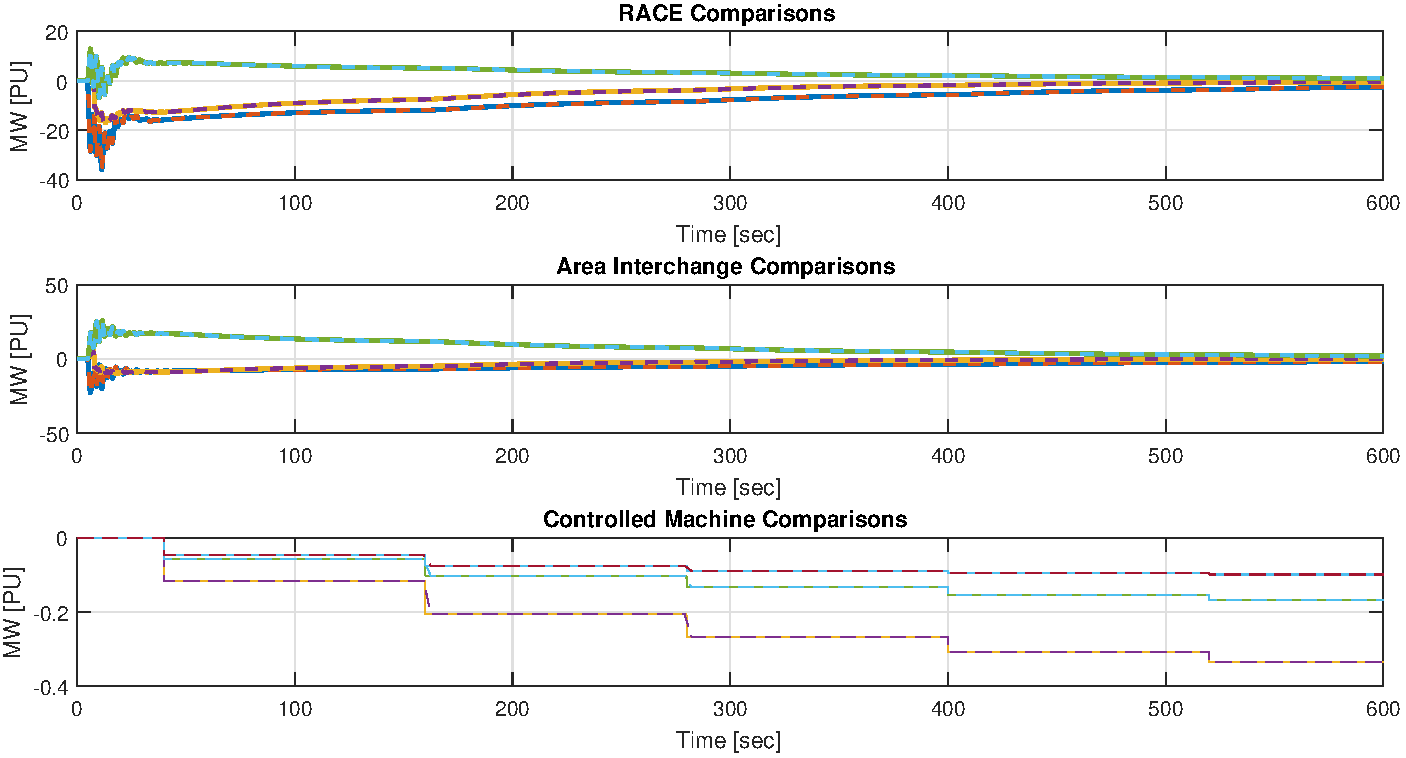
\includegraphics[width=\linewidth]{examples/miniWECC/mwAGC-AGCcalcs}
	\caption{MiniWECC AGC recovery FTS vs VTS AGC values.}
	\label{fig: mwAGC agc values}
\end{figure}%\vspace{-1 em}